\section{Estadísticos muestrales}

\begin{ejercicio}
    Sea $(X_1, \ldots, X_n)$ una muestra aleatoria simple de una variable aleatoria $X$. Dar el espacio muestral y calcular la función masa de probabilidad de $(X_1, \ldots, X_n)$ en cada uno de los siguientes casos:
    \begin{enumerate}[label=\alph*)]
        \item $X\rightsquigarrow \{B(k_0,p) : p\in (0,1)\}$ Binomial.

            El espacio muestral en este caso es $\cc{X}^n$, donde:
            \begin{equation*}
                \cc{X} = \{0, 1, ..., k_0\}
            \end{equation*}
            Recordamos que si $X\rightsquigarrow B(k_0,p)$, entonces:
            \begin{equation*}
                P[X=x] = \binom{k_0}{x} p^x {(1-p)}^{k_0-x} \qquad \forall x\in \cc{X}
            \end{equation*}
            Por tanto, para nuestra m.a.s. tendremos la función masa de probabilidad:
            \begin{align*}
                P[X_1 &= x_1, \ldots, X_n = x_n] \stackrel{\text{indep.}}{=} \prod_{i=1}^{n}P[X_i = x_i]\stackrel{\text{id. d.}}{=} \prod_{i=1}^{n} P[X=x_i] \\
                      &= \prod_{i=1}^{n} \binom{k_0}{x_i} p^{x_i} {(1-p)}^{k_0-x_i} = p^{\sum\limits_{i=1}^{n}x_i} {(1-p)}^{nk_0 - \sum\limits_{i=1}^{n}x_i} \prod_{i=1}^{n}\binom{k_0}{x_i} \\
                      & \qquad \forall (x_1, \ldots, x_n) \in \cc{X}^n
            \end{align*}
        \item $X\rightsquigarrow\{\cc{P}(\lm) : \lm \in \mathbb{R}^+\}$ Poisson.

            El espacio muestral de $X$ es:
            \begin{equation*}
                \cc{X} = \mathbb{N} \cup \{0\}
            \end{equation*} 
            Recordamos que si $X\rightsquigarrow \cc{P}(\lm)$, entonces:
            \begin{equation*}
                P[X=x] = e^{-\lm} \dfrac{\lm^x}{x!} \qquad \forall x\in \cc{X}
            \end{equation*}
            Por tanto:
            \begin{align*}
                P[X_1 &= x_1, \ldots, X_n = x_n] \stackrel{\text{indep.}}{=} \prod_{i=1}^{n}P[X_i = x_i]\stackrel{\text{id. d.}}{=} \prod_{i=1}^{n} P[X=x_i] \\
                      &= \prod_{i=1}^{n} e^{-\lm} \dfrac{\lm^{x_i}}{x_i!} = e^{-n\lm} \prod_{i=1}^{n} \dfrac{\lm^{x_i}}{x_i!} = e^{-n\lm} \cdot \dfrac{\lm^{\sum\limits_{i=1}^n x_i}}{\prod\limits_{i=1}^{n}x_i}  \qquad \forall (x_1, \ldots, x_n) \in \cc{X}^n
            \end{align*}
        \item $X\rightsquigarrow\{BN(k_0,p) : p\in (0,1)\}$ Binomial Negativa.

            El espacio muestral de $X$ es:
            \begin{equation*}
                \cc{X} = \mathbb{N}\cup \{0\}
            \end{equation*}
            Recordamos que si $X\rightsquigarrow BN(k_0,p)$, entonces:
            \begin{equation*}
                P[X=x] = \binom{x+k_0-1}{x} {(1-p)}^{x}p^{k_0} \qquad \forall x\in \cc{X}
            \end{equation*}
            Por tanto:
            \begin{align*}
                P[X_1 &= x_1, \ldots, X_n = x_n] \stackrel{\text{indep.}}{=} \prod_{i=1}^{n}P[X_i = x_i]\stackrel{\text{id. d.}}{=} \prod_{i=1}^{n} P[X=x_i] \\
                      &= \prod_{i=1}^{n} \binom{x_i+k_0-1}{x_i}{(1-p)}^{x_i}p^{k_0} = p^{nk_0}{(1-p)}^{\sum\limits_{i=1}^n x_i} \prod_{i=1}^{n}\binom{x_i+k_0-1}{x_i} \\
                      &\forall (x_1,\ldots,x_n)\in \cc{X}^n
            \end{align*}
        \item $X\rightsquigarrow\{G(p) : p\in (0,1)\}$ Geométrica.

            El espacio muestral de $X$ es:
            \begin{equation*}
                \cc{X} = \mathbb{N}\cup \{0\}
            \end{equation*}
            Recordamos que $G(p)\equiv BN(1,p)$, por lo que si sustituimos en la fórmula obtenida en la Binomial Negativa $k_0 = 1$:
            \begin{equation*}
                P[X_1=x_1, \ldots, X_n = x_n] = p^{n}{(1-p)}^{\sum\limits_{i=1}^n x_i} \qquad \forall (x_1,\ldots,x_n)\in \cc{X}^n
            \end{equation*}
        \item $X\rightsquigarrow\{P_N : N\in \mathbb{N}\}$, $\quad P_N(X=x) = \dfrac{1}{N}$, $\quad x=1,\ldots,N$.

            El espacio muestral ya nos lo dan: $\cc{X} = \{1,\ldots,N\}$. Calculemos la masa de probabilidad:
            \begin{align*}
                P[X_1 &= x_1, \ldots, X_n = x_n] \stackrel{\text{indep.}}{=} \prod_{i=1}^{n}P[X_i = x_i]\stackrel{\text{id. d.}}{=} \prod_{i=1}^{n} P[X=x_i] \\
                      &= \prod_{i=1}^{n} \dfrac{1}{N} = {\left(\dfrac{1}{N}\right)}^{n} \qquad \forall (x_1,\ldots,x_n) \in \cc{X}^n
            \end{align*}
    \end{enumerate}
\end{ejercicio}

\begin{ejercicio}
    Sea $(X_1, \ldots, X_n)$ una muestra aleatoria simple de una variable aleatoria $X$. Dar el espacio muestral y calcular la función de densidad de $(X_1, \ldots, X_n)$ en cada uno de los siguientes casos:
    \begin{enumerate}[label=\alph*)]
        \item $X\rightsquigarrow\{U(a,b) : a,b\in \mathbb{R}, a<b\}$ Uniforme.

            El espcio muestral en este caso es $\cc{X}^n$, donde:
            \begin{equation*}
                \cc{X} = [a,b]
            \end{equation*}
            Recordamos que si $X\rightsquigarrow U(a,b)$, entonces:
            \begin{equation*}
                f_X(x) = \dfrac{1}{b-a} \qquad \forall x\in [a,b]
            \end{equation*}
            Por lo que:
            \begin{align*}
                f_{(X_1, \ldots, X_n)}(x_1, \ldots, x_n) &\stackrel{\text{indep.}}{=} \prod_{i=1}^{n} f_{X_i}(x_i) \stackrel{\text{id. d.}}{=} \prod_{i=1}^{n} f_X(x_i) = \prod_{i=1}^{n} \dfrac{1}{b-a} \\ &= {\left(\dfrac{1}{b-a}\right)}^{n} \qquad \forall (x_1, \ldots, x_n) \in \cc{X}^n
            \end{align*}

        \item $X\rightsquigarrow\{\cc{N}(\mu, \sigma^2) : \mu \in \mathbb{R}, \sigma^2 \in \mathbb{R}^+\}$ Normal.

            El espacio muestral de $X$ es $\cc{X} = \mathbb{R}$. Recordamos que si $X\rightsquigarrow \cc{N}(\mu, \sigma^2)$, entonces:
            \begin{equation*}
                f_X(x) = \dfrac{1}{\sqrt{2\pi} \sigma} e^{-\dfrac{{(x-\mu)}^{2}}{2\sigma^2}} \qquad \forall x\in \mathbb{R}
            \end{equation*}
            Por lo que:
            \begin{align*}
                f_{(X_1, \ldots, X_n)}(x_1, \ldots, x_n) &\stackrel{\text{indep.}}{=} \prod_{i=1}^{n} f_{X_i}(x_i) \stackrel{\text{id. d.}}{=} \prod_{i=1}^{n} f_X(x_i) 
                = \prod_{i=1}^{n} \dfrac{1}{\sqrt{2\pi} \sigma} e^{-\dfrac{{(x_i-\mu)}^{2}}{2\sigma^2}}  \\
                &= {\left(\dfrac{1}{\sqrt{2\pi}\sigma}\right)}^{n} \prod_{i=1}^{n} e^{-\dfrac{{(x_i-\mu)}^{2}}{2\sigma^2}}  = {\left(\dfrac{1}{\sqrt{2\pi}\sigma}\right)}^{n} e^{-\sum\limits_{i=1}^n\dfrac{{(x_i-\mu)}^{2}}{2\sigma^2}}   \\
                &= {\left(\dfrac{1}{\sqrt{2\pi}\sigma}\right)}^{n} e^{\frac{-1}{2\sigma^2}\sum\limits_{i=1}^n {(x_i-\mu)}^{2}} \qquad \forall (x_1,\ldots,x_n) \in \mathbb{R}^n
            \end{align*}
        \item $X\rightsquigarrow\{\Gamma(p,a) : p,a\in \mathbb{R}^+\}$ Gamma.

            El espacio muestral de $X$ es $\cc{X}=\mathbb{R}^+_0$. Recordamos que si $X\rightsquigarrow \Gamma(p,a)$, entonces:
            \begin{equation*}
                f_X(x) = \dfrac{a^p}{\Gamma(p)} x^{p-1} e^{-ax} \qquad \forall x\in \mathbb{R}^+_0
            \end{equation*}
            Por lo que:
            \begin{align*}
                f_{(X_1, \ldots, X_n)}(x_1, \ldots, x_n) &\stackrel{\text{indep.}}{=} \prod_{i=1}^{n} f_{X_i}(x_i) \stackrel{\text{id. d.}}{=} \prod_{i=1}^{n} f_X(x_i) 
                = \prod_{i=1}^{n} \dfrac{a^p}{\Gamma(p)} x_i^{p-1} e^{-ax_i} \\
                                                         &= {\left(\dfrac{a^p}{\Gamma(p)}\right)}^{n} \cdot e^{-a\sum\limits_{i=1}^n x_i} \cdot \prod_{i=1}^{n} x_i^{p-1} \qquad \forall (x_1,\ldots,x_n)\in \cc{X}^n
            \end{align*}
        \item $X\rightsquigarrow\{\beta(p,q) : p,q\in \mathbb{R}^+\}$ Beta.

            El espacio muestral de $X$ es $\cc{X} = [0,1]$. Recordamos que si $X\rightsquigarrow \beta(p,q)$, entonces:
            \begin{equation*}
                f_X(x) = \dfrac{1}{\beta(p,q)} x^{p-1} {(1-x)}^{q-1} \qquad \forall x\in [0,1]
            \end{equation*}
            Donde:
            \begin{equation*}
                \beta(p,q) = \dfrac{\Gamma(p)\Gamma(q)}{\Gamma(p+q)}
            \end{equation*}
            Por tanto:
            \begin{align*}
                f_{(X_1, \ldots, X_n)}(x_1, \ldots, x_n) &\stackrel{\text{indep.}}{=} \prod_{i=1}^{n} f_{X_i}(x_i) \stackrel{\text{id. d.}}{=} \prod_{i=1}^{n} f_X(x_i) 
                = \prod_{i=1}^{n} \dfrac{1}{\beta(p,q)} x_i^{p-1} {(1-x_i)}^{q-1} \\
                                                         &= \dfrac{1}{{\beta(p,q)}^{n}} \prod_{i=1}^{n}x_i^{p-1} {(1-x_i)}^{q-1} \qquad \forall (x_1,\ldots,x_n) \in \cc{X}^n
            \end{align*}
        \item $X\rightsquigarrow\{P_\theta : \theta \in \mathbb{R}^+\}$, $\quad f_\theta(x) = \dfrac{1}{2\sqrt{x\theta}}$, $\quad 0<x<\theta$.

            Se nos dice que $\cc{X} = \left]0,\theta\right[$. Calculamos la función de densidad conjunta:
            \begin{align*}
                f_{(X_1, \ldots, X_n)}(x_1, \ldots, x_n) &\stackrel{\text{indep.}}{=} \prod_{i=1}^{n} f_{X_i}(x_i) \stackrel{\text{id. d.}}{=} \prod_{i=1}^{n} f_X(x_i) 
                = \prod_{i=1}^{n} \dfrac{1}{2\sqrt{x_i \theta}} \\
                                                         &= \dfrac{1}{{\left(2\sqrt{\theta}\right)}^{n}} \prod_{i=1}^{n} \dfrac{1}{\sqrt{x_i}} \qquad \forall (x_1, \ldots, x_n) \in  \cc{X}^n
            \end{align*}
    \end{enumerate}
\end{ejercicio}

\begin{ejercicio}
    Se miden los tiempos de sedimentación de una muestra de partículas flotando en un líquido. Los tiempos observados son: 
    \begin{gather*}
        11.5; 1.8; 7.3; 12.1; 1.8; 21.3; 7.3; 15.2; 7.3; 12.1; 15.2;\\ 7.3; 12.1; 1.8; 10.5; 15.2; 21.3; 10.5; 15.2; 11.5
    \end{gather*}
    \begin{itemize}
        \item Construir la función de distribución muestral asociada a a dichas observaciones.

            Si aplicamos la definición de función de distribución muestral obtenemos que esta viene dada por:
            \begin{equation*}
                F_n^\ast(x) =
                \begin{cases} 
                0 & \text{si\ } x < 1.8 \\[6pt]
                \nicefrac{3}{20} &\text{si\ } 1.8 \leq x < 7.3 \\[6pt]
                \nicefrac{7}{20} &\text{si\ } 7.3 \leq x < 10.5 \\[6pt]
                \nicefrac{9}{20} &\text{si\ } 10.5 \leq x < 11.5 \\[6pt]
                \nicefrac{11}{20} &\text{si\ } 11.5 \leq x < 12.1 \\[6pt]
                \nicefrac{14}{20} &\text{si\ } 12.1 \leq x < 15.2 \\[6pt]
                \nicefrac{18}{20} &\text{si\ } 15.2 \leq x < 21.3 \\[6pt]
                \nicefrac{20}{20} &\text{si\ } x \geq 21.3
                \end{cases}
            \end{equation*}

            \begin{figure}[H]
                \centering
                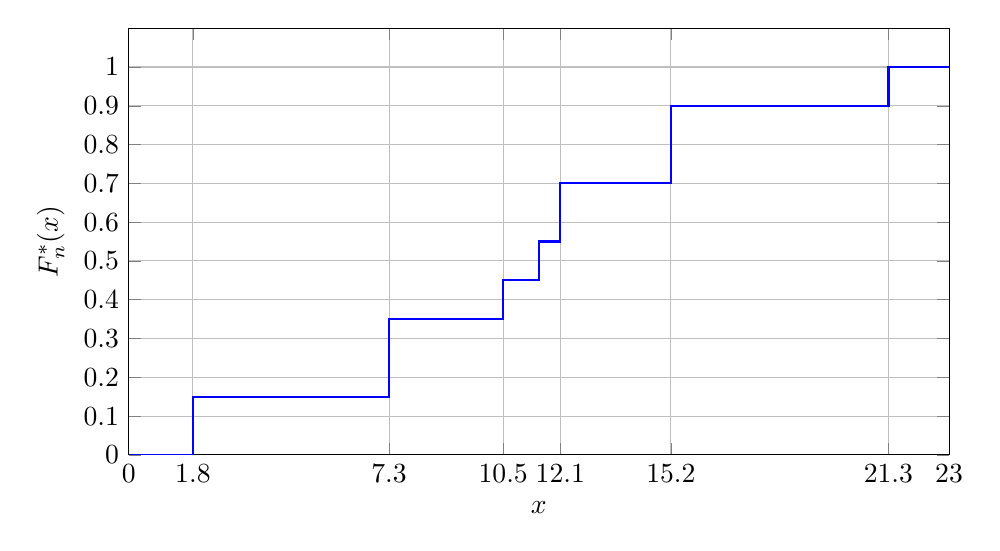
\begin{tikzpicture}
                \begin{axis}[
                    width=12cm, height=7cm, xlabel={$x$}, ylabel={$F_n^\ast(x)$}, ymin=0, ymax=1.1,
                    xmin=0, xmax=23, xtick={0,1.8,7.3,10.5,12.1,15.2,21.3,23},
                    ytick={0,0.1,0.2,0.3,0.4,0.5,0.6,0.7,0.8,0.9,1},
                    grid=both, domain=0:23, samples=200,
                ]

                % Graficamos la función escalonada
                \addplot[
                    thick, blue
                ] coordinates {
                    (0,0) (1.8,0) (1.8,3/20) (7.3,3/20) (7.3,7/20) (10.5,7/20)
                    (10.5,9/20) (11.5,9/20) (11.5,11/20) (12.1,11/20) (12.1,14/20)
                    (15.2,14/20) (15.2,18/20) (21.3,18/20) (21.3,20/20) (23,20/20)
                };
                \end{axis}
                \end{tikzpicture}
                \caption{Gráfica de la función de distribución muestral.}
            \end{figure}
        \item Hallar los valores de los tres primeros momentos muestrales respecto al origen y respecto a la media.

            Calculamos primero los tres primeros momentos respecto al origen para luego calcular los centrados respecto a la media a partir de ellos:
            \begin{align*}
                a_1 &= \sum_{i=1}^{n} f_i x_i = 10.915 \qquad 
                a_2 = \sum_{i=1}^{n} f_i x_i^2 = 148.9325 \\
                a_3 &= \sum_{i=1}^{n} f_i x_i^3 = 2280.98365 \\
                b_1 &= \sum_{i=1}^{n} f_i {(x_i - \overline{x})}= 0\qquad  \\
                b_2 &= \frac{1}{n}\sum_{i=1}^{n}{(x_i-\overline{x})}^{2} = \frac{1}{n}\sum_{i=1}^{n}(x_i^2 - 2x_i \overline{x}+\overline{x}^2)  \\ &= \frac{1}{n}\sum_{i=1}^{n}x_i^2 - \frac{2\overline{x}}{n}\sum_{i=1}^{n}x_i + \overline{x}^2 = a_2 -2a_1^2 + a_1^2 = a_2 - a_1^2 \\
                    &= 148.9325 - 10.915  = 29.795275\\
                b_3 &= \frac{1}{n}\sum_{i=1}^{n} {(x_i-\overline{x})}^{3} = \frac{1}{n}\sum_{i=1}^{n}\left(x_i^3 - 3x_i^2 \overline{x} + 3x_i\overline{x}^2 -\overline{x}^3\right) \\
                    &= \frac{1}{n}\sum_{i=1}^{n}x_i^3 - \frac{3\overline{x}}{n}\sum_{i=1}^{n}x_i^2 + \frac{3\overline{x}^2}{n}\sum_{i=1}^{n}x_i - \overline{x}^3 = a_3 - 3a_1a_2 + 3a_1^3 - a_1^3 \\
                    &= a_3 - 3a_1a_2 + 2a_1^3 = 4.95455925
            \end{align*}
        \item Determinar los valores de los cuartiles muestrales y el percentil 70.

            Para ello, primero ordenamos los datos de menor a mayor y los agrupamos en grupos de $\nicefrac{20}{4} = 5$ en 5:
            \begin{gather*}
                1.8;\ 1.8;\ 1.8;\ 7.3;\ 7.3;\ \red{7.3;\ 7.3;\ 10.5;\ 10.5;\ 11.5};\ 11.5;\ 12.1;\ 12.1;\\ 12.1;\ 15.2;\ \red{15.2;\ 15.2;\ 15.2;\ 21.3;\ 21.3}
            \end{gather*}
            Como en los cambios de agrupaciones de números estos se repiten, hemos obtenido el valor de los cuartiles:
            \begin{equation*}
                q_1 = 7.3 \qquad q_2 = 11.5 \qquad q_3 = 15.2 \qquad q_4 = 21.3
            \end{equation*}
            Para el percentil $70$, calculamos:
            \begin{equation*}
                0.7\cdot 20 = 14
            \end{equation*}
            Como hemos obtenido un número entero, el percentil 70 será:
            \begin{equation*}
                c_{70} = \dfrac{X_{(14)} + X_{(15)}}{2} = \dfrac{12.1 + 15.2}{2} = 13.65
            \end{equation*}
            En el caso de haber obtenido un número no entero (por ejemplo, $14.2$), sería $X_{(15)}$.
    \end{itemize}
\end{ejercicio}

\begin{ejercicio}
    Se dispone de una muestra aleatoria simple de tamaño 40 de una distribución exponencial de media 3, ¿cuál es la probabilidad de que los valores de la función de distribución muestral y la teórica, en $x=1$, difieran menos de $0.01$? Aproximadamente, ¿cuál debe ser el tamaño muestral para que dicha probabilidad sea como mínimo $0.98$?\\

    \noindent
    Como dice el enunciado, tenemos una m.a.s. $(X_1, \ldots, X_n)$ con $n=40$, todas ellas idénticamente distribuidas a $X\rightsquigarrow exp(\lm)$. Sabemos de la asignatura de Probabilidad que:
    \begin{equation*}
        E[X] = \dfrac{1}{\lm} = 3 \Longrightarrow \lm = \dfrac{1}{3}
    \end{equation*}
    Por lo que $X\rightsquigarrow exp\left(\frac{1}{3}\right)$. Denotaremos por comodidad:
    \begin{equation*}
        F_n^\ast(x) = F_{(X_1, \ldots, X_n)}^\ast(x) 
    \end{equation*}
    Y el enunciado nos pregunta por:
    \begin{equation*}
        P[|F_n^\ast(1) - F_X(1)| < 0.01]
    \end{equation*}
    Para ello, primero calculamos $F_X(1)$:
    \begin{equation*}
        F_X(1) = 1 - e^{-\lm\cdot  1} = 1-e^{-\lm} = 1-e^{-\nicefrac{1}{3}} = \alpha
    \end{equation*}
    Por lo que nos disponemos ya a calcular la probabilidad:
    \begin{align*}
        P[|F_n^\ast(1) - F_X(1)| < 0.01] &= P[|F_n^\ast(1) - \alpha| < 0.01] = P[-0.01 < F_n^\ast(1) - \alpha < 0.01] \\
                                         &= P[-0.01+\alpha < F_n^\ast(1) < 0.01+\alpha] \\
                                         &= P[40(-0.01+\alpha) < 40F_n^\ast(1) < 40(0.01+\alpha)]
    \end{align*}
    Y como sabemos que $Y = 40F_n^\ast(1) \rightsquigarrow B(40, F_X(1)) \equiv B(40, \alpha)$:
    \begin{equation*}
        P[|F_n^\ast(1) - F_X(1)| < 0.01] = P[40(-0.01+\alpha) < Y< 40(0.01+\alpha)] 
    \end{equation*}
    Si ahora tomamos:
    \begin{equation*}
        \alpha = 1-e^{-\nicefrac{1}{3}}\approx 0.283469
    \end{equation*}
    Entonces:
    \begin{align*}
        40(0.01 + \alpha) &\approx 40(0.01+0.283469)= 11.73876 \\
        40(-0.01 + \alpha) &\approx 40(-0.01 + 0.283469)  = 10.93876
    \end{align*}
    Por lo que:
    \begin{align*}
        P[|F_n^\ast(1) - F_X(1)| < 0.01] &\approx P[10.93876 < Y < 11.73876] = P[Y=11]
    \end{align*}
    De donde usando la masa de probabilidad de la Binomial:
    \begin{equation*}
        P[Y=11] = \binom{40}{11} {(0.283469)}^{11} {(1-0.283469)}^{40-11} \approx 0.139
    \end{equation*}

    \noindent
    Para el segundo apartado, como para $n=40$ obtenemos una probabilidad de $0.139$, podemos intuir que para que dicha probabilidad sea como mínimo $0.98$, nos es necesario un valor de $n$ grande, por lo que podemos suponer que:
    \begin{equation*}
        F_n^\ast(1) \rightsquigarrow \cc{N}\left(\alpha, \dfrac{\alpha(1-\alpha)}{n}\right)
    \end{equation*}
    De donde:
    \begin{equation*}
        Z = \dfrac{\sqrt{n}(F_n^\ast(1)-\alpha)}{\sqrt{\alpha(1-\alpha)}} \rightsquigarrow \cc{N}(0,1)
    \end{equation*}
    Buscamos el valor de $n$ que verifica:
    \begin{equation*}
        0.98 \leq P[|F_n^\ast(1) - F_X(1)| < 0.01] = P\left[|Z| < \dfrac{\sqrt{n}0.01}{\sqrt{\alpha(1-\alpha)}}\right]
    \end{equation*}
    Si aplicamos propiedades conocidas de la Normal, si $a\in \mathbb{R}$, entonces:
    \begin{equation*}
        P[|Z| < a] = P[-a < Z < a] = P[Z<a] - P[Z< -a]
    \end{equation*}
    Pero:
    \begin{equation*}
        P[Z< -a] = P[Z>a] = 1-P[Z-a]
    \end{equation*}
    Por lo que:
    \begin{equation*}
        P[|Z| < a] = P[Z<a] - P[Z < -a] = 2P[Z<a] - 1
    \end{equation*}
    Volviendo al caso que nos interesa:
    \begin{equation*}
        0.98 \leq P\left[|Z| < \dfrac{\sqrt{n}0.01}{\sqrt{\alpha(1-\alpha)}}\right] = 2P\left[Z<\dfrac{\sqrt{n}0.01}{\sqrt{\alpha(1-\alpha)}}\right] - 1
    \end{equation*}
    Luego:
    \begin{equation*}
        0.99 = \dfrac{0.98+1}{2} \leq P\left[Z < \dfrac{\sqrt{n}0.01}{\sqrt{\alpha(1-\alpha)}}\right]
    \end{equation*}
    Si consultamos la tabla de la normal $\cc{N}(0,1)$, observamos que el primer valor que supera la probbailidad de $0.99$ es $2.33$, por lo que:
    \begin{equation*}
        2.33 = \dfrac{\sqrt{n}0.01}{\sqrt{\alpha(1-\alpha)}} = \dfrac{\sqrt{n}0.01}{\sqrt{0.283469(1-0.283469)}} \approx 0.0221886 \sqrt{n}
    \end{equation*}
    De donde:
    \begin{equation*}
        5.4289 = {(2.33)}^{2} = {(0.0221886\sqrt{n})}^{2} = 0.00049233 n \Longrightarrow n = \dfrac{5.4289}{0.00049233} = 11026.95347
    \end{equation*}
    Por lo que para $n \geq 11027$ podemos asegurar que la probabilidad es como mínimo $0.98$.
\end{ejercicio}

\begin{ejercicio}
    Se dispone de una muestra aleatoria simple de tamaño 50 de una distribución de Poisson de media 2, ¿cuál es la probabilidad de que los valores de la función de distribución muestral y la teórica, en $x=2$, difieran menos de $0.02$? Aproximadamente, ¿qué tamaño muestral hay que tomar para que dicha probabilidad sea como mínimo $0.99$?\\

    \noindent
    Tenemos una m.a.s. $(X_1, \ldots, X_n)$ con $n=50$ idénticamente distribuidas a $X\rightsquigarrow \cc{P}(2)$. Notamos por comodidad:
    \begin{equation*}
        F_{(X_1, \ldots, X_n)}^\ast(x) = F_n^\ast(x)
    \end{equation*}
    Nos preguntan por:
    \begin{equation*}
        P[|F_n^\ast(2) - F_X(2)| < 0.02]
    \end{equation*}
    Para ello primero calculamos:
    \begin{equation*}
        F_X(2) = \sum_{k=0}^{2} e^{-2}\dfrac{2^k}{k!} =  e^{-2}\left(\dfrac{2^0}{0!} + \dfrac{2^1}{1!} + \dfrac{2^2}{2!}\right) = e^{-2} (1+2+2) \approx 0.6767
    \end{equation*}
    Por lo que:
    \begin{equation*}
        P[|F_n^\ast(2) - 0.6767| < 0.02] = P[-0.02 < F_n^\ast(2) - 0.6767 < 0.02] = P[0.6567 < F_n^\ast(2) < 0.6967]
    \end{equation*}
    Como sabemos por lo visto en teoría que:
    \begin{equation*}
        Y = 50F_n^\ast(2) \rightsquigarrow B(50, F_X(2)) \equiv B(50,\ \ 0.6767)
    \end{equation*}
    Multiplicamos por $50$ la última expresión:
    \begin{align*}
        P[|F_n^\ast(2) - 0.6767| < 0.02] = P[0.6567 < F_n^\ast(2) < 0.6967] &= P[32.835 < Y< 34.835] \\
                                         &= P[Y = 33] + P[Y=34]
    \end{align*}
    Y calculamos estas dos probabilidades:
    \begin{align*}
        P[Y=33] &= \binom{50}{33} {(0.6767)}^{33} {(1-0.6767)}^{50-33} \approx 0.114734\\
        P[Y=34] &= \binom{50}{34} {(0.6767)}^{34} {(1-0.6767)}^{50-34} \approx 0.120075
    \end{align*}
    Por lo que:
    \begin{equation*}
        P[|F_n^\ast(2) - 0.6767| < 0.02] \approx 0.114734 + 0.120075 = 0.234809
    \end{equation*}

    \noindent
    Para el segundo apartado, como para $n=50$ obtenemos una probabilidad de $0.234809$, podemos intuir que para que dicha probabilidad sea como mínimo $0.99$, nos es necesario un valor de $n$ grande, por lo que podemos suponer que:
    \begin{equation*}
        F_n^\ast(2) \rightsquigarrow \cc{N}\left(0.6767, \dfrac{0.6767(1-0.6767)}{n}\right) \equiv \cc{N}\left(0.6767, \dfrac{0.218777}{n}\right)
    \end{equation*}
    Por lo que:
    \begin{equation*}
        Z = \dfrac{\sqrt{n}(F_n^\ast(2) - 0.6767)}{\sqrt{0.218777}} \rightsquigarrow\cc{N}(0,1)
    \end{equation*}
    En dicho caso, buscamos $n$ de forma que:
    \begin{equation*}
        0.99 \leq P[|F_n^\ast(2) - F_X(2)| < 0.02] = P\left[|Z| < \dfrac{\sqrt{n}0.02}{\sqrt{0.218777}}\right]
    \end{equation*}
    De forma análoga al ejercicio anterior:
    \begin{equation*}
        P\left[|Z| < \dfrac{\sqrt{n}0.02}{\sqrt{0.218777}}\right] = 2P\left[Z < \dfrac{\sqrt{n}0.02}{\sqrt{0.218777}}\right] - 1
    \end{equation*}
    Luego:
    \begin{equation*}
        0.995 = \dfrac{0.99 + 1}{2} \leq P\left[Z < \dfrac{\sqrt{n}0.02}{\sqrt{0.218777}}\right] 
    \end{equation*}
    Y si miramos la tabla de la Normal observamos que el primer valor que supera la probabilidad de $0.995$ es $2.58$, luego:
    \begin{equation*}
        2.58 = \dfrac{\sqrt{n}0.02}{\sqrt{0.218777}} = 0.042759 \sqrt{n}
    \end{equation*}
    Por lo que:
    \begin{equation*}
        6.6564 = {(2.58)}^{2} = {(0.042759 \sqrt{n})}^{2} = 0.00182833 n
    \end{equation*}
    Luego:
    \begin{equation*}
        n = \dfrac{6.6564}{0.00182833} \approx 3640.7
    \end{equation*}
    Por lo que para $n\geq 3641$ podemos asegurar que la probabilidad es como mínimo $0.99$.
\end{ejercicio}

\begin{ejercicio}
   Sea $X\rightsquigarrow B(1,p)$ y $(X_1, X_2, X_3)$ una muestra aleatoria simple de $X$. Calcular la función masa de probabilidad de los estadísticos $\overline{X}$, $S^2$, $\min X_i$ y $\max X_i$.\\

   \noindent
   Para resolver este ejercicio, como $X$ sigue una distribución discreta, buscamos aplicar el teorema de cambio de variable de discreta a discreta. Para ello, la forma más cómoda será analizar cada uno de los valores que puede tomar la muestra aleatoria simple $(X_1, X_2, X_3)$ y determinar en consecuencia cada uno de los valores que toman $\overline{X}$, $S^2$, $\min X_i$ y $\max X_i$. Acompañaremos la tabla junto con la probabilidad de que la muestra tome dicho valor, es decir, en la fila correpondiente a $(x_1, x_2, x_3)$ incluiremos $P[X_1 = x_1, X_2 = x_2, X_3 = x_3]$:
   \begin{equation*}
   \begin{array}{c|c|c|c|c|c}
       P & (X_1, X_2, X_3) & \overline{X} & S^2 & \min X_i & \max X_i  \\
       \hline
       {(1-p)}^{3} & (0,0,0) & 0 & 0 & 0 & 0 \\
       p{(1-p)}^{2} & (0,0,1) & \nicefrac{1}{3} & \nicefrac{1}{3} & 0 & 1 \\
       p{(1-p)}^{2} & (0,1,0) & \nicefrac{1}{3} & \nicefrac{1}{3} & 0 & 1 \\
       p^2(1-p) & (0,1,1) & \nicefrac{2}{3} & \nicefrac{1}{3} & 0 & 1 \\
       p{(1-p)}^{2} & (1,0,0) & \nicefrac{1}{3} & \nicefrac{1}{3} & 0 & 1 \\
       p^2(1-p) & (1,0,1) & \nicefrac{2}{3} & \nicefrac{1}{3} & 0 & 1 \\
       p^2(1-p) & (1,1,0) & \nicefrac{2}{3} & \nicefrac{1}{3} & 0 & 1 \\
       p^3 & (1,1,1) & 1 & 0 & 1 & 1 
   \end{array}
   \end{equation*}
   Podemos ya calcular la función masa de probabilidad de cada uno de los estadísticos, simplemente sumando las probabilidades de la tabla que corresponden a cada valor del espacio muestral de cada estadístico:
   \begin{itemize}
       \item Para $\overline{X}$:
           \begin{align*}
               P[\overline{X} = 0] &= P[X_1 = 0, X_2 = 0, X_3=0] = {(1-p)}^{3}  \\
               P[\overline{X} = \nicefrac{1}{3}] &= \sum_{i=1}^{3}p{(1-p)}^{2} = 3p{(1-p)}^{2} \\
               P[\overline{X} = \nicefrac{2}{3}] &= \sum_{i=1}^{3}p^2(1-p) = 3p^2(1-p) \\
               P[\overline{X} = 1] &= P[X_1 = 1, X_2 = 1, X_3 = 1] = p^3
           \end{align*}
       \item Para $S^2$:
           \begin{align*}
               P[S^2 = 0] &= P[X_1 = 0, X_2 = 0, X_3 = 0] + P[X_1 = 1, X_2 = 1, X_3 = 1] = p^3 + {(1-p)}^{3} \\
               P[S^2 = \nicefrac{1}{3}] &= \sum_{i=1}^{3} p{(1-p)}^{2} + \sum_{i=1}^{3}p^2(1-p) = 3p(1-p)(p+1-p) = 3p(1-p)
           \end{align*}
       \item Para $\min X_i$:
           \begin{align*}
               P[\min X_i = 1] &= P[X_1 = 1, X_2 = 1, X_3 = 1] = p^3 \\
               P[\min X_i = 0] &= 1-P[\min X_i = 1] = 1-p^3
           \end{align*}
       \item Para $\max X_i$:
           \begin{align*}
               P[\max X_i = 0] &= P[X_1 = 0, X_2 = 0, X_3 = 0] = {(1-p)}^{3}\\
               P[\max X_i = 1] &= 1-P[\max X_i = 0] = 1-{(1-p)}^{3}
           \end{align*}
   \end{itemize}
\end{ejercicio}

\begin{ejercicio}
    Obtener la función masa de probabilidad o función de densidad de $\overline{X}$ en el muestreo de una variable de Bernoulli, de una Poisson y de una exponencial.\\

    \noindent
    Calculamos la masa de probabilidad o función de densidad en cada caso, suponiendo que tenemos $(X_1, \ldots, X_n)$ una muestra aleatoria simple con variables aleatorias idénticamente distribuidas a $X$, que sigue una distribución distinta en cada caso y estaremos interesados en calcular la masa de:
    \begin{equation*}
        \overline{X} = \sum_{i=1}^{n}
    \end{equation*}
    \begin{description}
        \item [Bernoulli.] Supuesto que $X\rightsquigarrow B(1,p)$ para cierto $p\in \left]0,1\right[$, si tomamos:
            \begin{equation*}
                Y = \sum_{i=1}^{n}X_i
            \end{equation*}
            Por la propiedad reproductiva de la Bernoulli, tenemos que $Y\rightsquigarrow B(n,p)$. En dicho caso:
            \begin{equation*}
                P[Y=k] = \binom{n}{k} p^k {(1-p)}^{n-k} \qquad \forall k\in \{0,\ldots,n\}
            \end{equation*}
            Por tanto, tendremos que:
            \begin{equation*}
                P\left[\overline{X} = \frac{k}{n}\right] = P[Y=k] = \binom{n}{k} p^k {(1-p)}^{n-k} \qquad \forall k\in \{0,\ldots,n\}
            \end{equation*}
        \item [Poisson.] Supuesto que $X\rightsquigarrow \cc{P}(\lm)$ para cierto $\lm\in \mathbb{R}^+$, si tomamos:
            \begin{equation*}
                Y = \sum_{i=1}^{n}X_i
            \end{equation*}
            Por la propiedad reproductiva de la Poisson, tendremos que:
            \begin{equation*}
                Y\rightsquigarrow\cc{P}\left(\sum_{i=1}^{n}\lm\right) \equiv \cc{P}(n\lm)
            \end{equation*}
            En dicho caso:
            \begin{equation*}
                P[Y=x] = e^{-n\lm} \dfrac{{(n\lm)}^{x}}{x!} \qquad \forall x\in \mathbb{N}
            \end{equation*}
            Por lo que:
            \begin{equation*}
                P[\overline{X}=\nicefrac{x}{n}] = P[Y=x] = e^{-n\lm} \dfrac{{(n\lm)}^{x}}{x!} \qquad \forall x\in \mathbb{N}
            \end{equation*}
        \item [Exponencial.] Supuesto ahora que $X\rightsquigarrow exp(\lm)$ para cierto $\lm\in \mathbb{R}^+$, tendremos entonces que:
            \begin{equation*}
                M_X(t) = \dfrac{\lm}{\lm - t} \qquad t<\lm
            \end{equation*}
            Si aplicamos la igualdad $(\ast)$ vista en teoría:
            \begin{align*}
                M_{\overline{X}}(t) &\AstIg {(M_X(\nicefrac{t}{n}))}^{n} = {\left(\dfrac{\lm}{\lm - \nicefrac{t}{n}}\right)}^{n} = {\left(\dfrac{n\lm}{n\lm - t}\right)}^{n}
            \end{align*}
            Observamos que obtenemos una función generatriz de momentos para $\overline{X}$ igual que para una variable aleatoria de distribución $\Gamma(n,n\lm)$. Como la función generatriz de momentos de una variable aleatoria caracteriza su distribución, concluimos que $\overline{X}\rightsquigarrow\Gamma(n,n\lm)$.
    \end{description}
\end{ejercicio}

\begin{ejercicio}
    Calcular las funciones de densidad de los estadísticos $\max X_i$ y $\min X_i$ en el muestreo de una variable $X$ con funcion de densidad:
    \begin{equation*}
        f_\theta(x) = e^{\theta-x}, \qquad x>\theta.
    \end{equation*}

    \noindent
    Calculamos primero la función de distribución, para calcular con mayor comodidad las funciones de distribución de $X_{(n)}$ y $X_{(1)}$:
    \begin{equation*}
        F_\theta(x) = \int_{\theta}^{x} f_\theta(t)~dt = \int_{\theta}^{x} e^{\theta-t}~dt  = \left[-e^{\theta-t}\right]_\theta^x = 1 - e^{\theta - x} \qquad \forall x\in \mathbb{R}^+
    \end{equation*}
    Supuesto ahora que disponemos de una m.a.s. $(X_1, \ldots, X_n)$ idénticamente distribuidas a $X$ cuya función de densidad es la anteriormente dicha, podemos aplicar las fórmulas obtenidas en teoría para calcular las funciones de distribución del mínimo y del máximo. Para el máximo:
    \begin{equation*}
        F_{X_{(n)}}(x) = {(F_X(x))}^{n} = {(1-e^{\theta-x})}^{n} \Longrightarrow f_{X_{(n)}} = n{(1-e^{\theta - x})}^{n-1}e^{\theta -x} \qquad \forall x\in \mathbb{R}^+
    \end{equation*}
    Para el mínimo:
    \begin{equation*}
        F_{X_{(1)}}(x) = 1 - {(1-F_X(n))}^{n} = 1-{(1-1+e^{\theta-x})}^{n} = 1-e^{n(\theta-x)} \qquad \forall x\in \mathbb{R}^+
    \end{equation*}
    de donde:
    \begin{equation*}
        f_{X_{(1)}}(x) = ne^{n(\theta-x)-1} \qquad \forall x\in \mathbb{R}^+
    \end{equation*}

\end{ejercicio}

\begin{ejercicio}
    El número de pacientes que visitan diariamente una determinada consulta médica es una variable aleatoria con varianza de 16 personas. Se supone que el número de visitas de cada día es independiente de cualquier otro. Si se observa el número de visitas diarias durante 64 días, calcular aproximadamente la probabilidad de que la media muestral no difiera en más de una persona del valor medio verdadero de visitas diarias.\\

    \noindent
    Sea $X$ una variable aleatoria que indica el número de pacientes que visitan diariamente dicha consulta médica, por cómo nos definen $X$ sabemos que $X\rightsquigarrow\cc{P}(\lm)$. Como además nos dicen que la varianza de dicha variable aleatoria es $16$, tenemos que $Var(X) = \lm = 16$. Si tenemos ahora una muestra aleatoria simple $(X_1, \ldots, X_n)$ con $n=64$, nos preguntan por:
    \begin{equation*}
        P[|\overline{X} - E[X]| < 1]
    \end{equation*}
    Donde $E[X] = \lm = 16$, ya que $X\rightsquigarrow\cc{P}(16)$. Calculamos:
    \begin{align*}
        P[|\overline{X} - E[X]| < 1] &= P[-1 < \overline{X}-16 < 1] = P[15 < \overline{X} < 17]
    \end{align*}
    Aplicamos ahora lo visto en el ejercicio 7, ya que si $X\rightsquigarrow\cc{P}(\lm)$, entonces tendremos que $n\overline{X}\rightsquigarrow \cc{P}(n\lm)$, gracias a la propiedad reproductiva de la Poisson:
    \begin{align*}
        P[|\overline{X} - E[X]| < 1] &= P[15 < \overline{X} < 17] = P[64\cdot 15 < 64\overline{X}<64\cdot 17] \\
                                     &= P[960 < 64\overline{X} < 1088]
    \end{align*}
    Donde $64\overline{X}\rightsquigarrow\cc{P}(64\cdot 16) \equiv \cc{P}(1024)$. Para calcular dicha probabilidad, aproximaremos la Poisson a una distribución normal:
    \begin{equation*}
        \cc{P}(1024) \approx \cc{N}(1024, 1024)
    \end{equation*}
    Por lo que:
    \begin{align*}
        P[|\overline{X} - E[X]| < 1] &= P[960 < 64\overline{X} < 1088] \approx P\left[\dfrac{960-1024}{\sqrt{1024}} < Z < \dfrac{1088 - 1024}{\sqrt{1024}}\right] \\
                                     &= P[-2 < Z < 2] = 2P[Z<2] -1  \\
                                     &= 2\cdot 0.97725 - 1 = 0.9545
    \end{align*}
\end{ejercicio}

\begin{ejercicio}   % // TODO: HACER
    Una máquina de refrescos está arreglada para que la cantidad de bebida que sirve sea una variable aleatoria con media 200 ml. y desviación típica 15 ml. Calcular de forma aproximada la probabilidad de que la cantidad media servida en una muestra aleatoria de tamaño 36 sea al menos 204 ml.\\

    \noindent
    \underline{\textbf{Suponiendo}} que la variable aleatoria que muestra la cantidad de bebida que sirve dicha máquina de refrescos es una variable aleatoria $X$ que sigue una distribución $\cc{N}(200, {15}^{2})$, consideramos una muestra aleatoria simple $(X_1, \ldots, X_n)$ de tamaño $n=36$ de variables idénticamente distribuidas a $X$, y queremos calcular:
    \begin{equation*}
        P[\overline{X}\geq 204]
    \end{equation*}
    En teoría hemos visto que bajo estas situaciones, se tiene que $\overline{X}\rightsquigarrow\cc{N}\left(200, \frac{15^2}{36}\right)$. Calculamos la probabilidad:
    \begin{align*}
        P[\overline{X}\geq 204] \stackrel{\text{tipificamos}}{=} P \left[Z \geq \dfrac{\sqrt{36}(204-200)}{15}\right] &= P[Z\geq 1.6] = 1 - P[Z< 1.6] \\
                                                                                                                      &= 1 - 0.9452 = 0.0548
    \end{align*}
\end{ejercicio}
